% Fig 2: nested-containment view of the simulability hierarchy (cleaner than ellipses).
\begin{figure}[t]
\centering
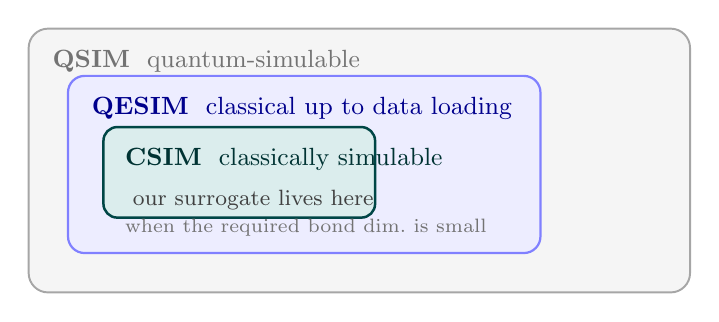
\begin{tikzpicture}[font=\small]
% outer: QSIM
\draw[rounded corners=7pt, draw=black!35, fill=black!4, line width=0.7pt] (0,0) rectangle (8.4,3.35);
\node[anchor=north west, black!55] at (0.18,3.2) {\textbf{QSIM}~~quantum-simulable};
% middle: QESIM
\draw[rounded corners=6pt, draw=blue!50, fill=blue!7, line width=0.8pt] (0.5,0.5) rectangle (6.5,2.75);
\node[anchor=north west, blue!55!black] at (0.68,2.6) {\textbf{QESIM}~~classical up to data loading};
% inner: CSIM
\draw[rounded corners=5pt, draw=teal!55!black, fill=teal!14, line width=0.9pt] (0.95,0.95) rectangle (4.4,2.1);
\node[anchor=north west, teal!40!black] at (1.1,1.95) {\textbf{CSIM}~~classically simulable};
\node[anchor=north west, black!75, font=\footnotesize] at (1.1,1.42) {$\bigstar$~our surrogate lives here};
\node[anchor=north west, black!55, font=\scriptsize] at (1.1,1.06) {when the required bond dim.\ is small};
\end{tikzpicture}
\caption{The nested hierarchy of classical simulability. A model that is classically simulable
(CSIM) is a special case of one that is simulable up to a data-loading step (QESIM), which in turn
is a special case of quantum-simulable (QSIM) \citep{cerezo2025,shin2024}. Our matrix-product-state
surrogate certifies membership in CSIM whenever the required bond dimension is small, and we make no
claim outside that innermost region.}
\label{fig:venn}
\end{figure}
